% !TEX root = autopaxos.tex
% !TEX TS-program = pdflatexmk
% For TeXShop on OS X and Herbert Schulz's latexmk engine.

\section{Evaluation}\label{evaluation}

\subsection{Measurement}
Our first task was to quantify the amount and character of information at our disposal.
After we wrapped all of the appropriate calls in instrumentation, we created a pair of experiments which set random environment constraints and then evaluated how accurately the system tracked those values.

% RTT tracking
\begin{figure}[htbp]
\begin{center}
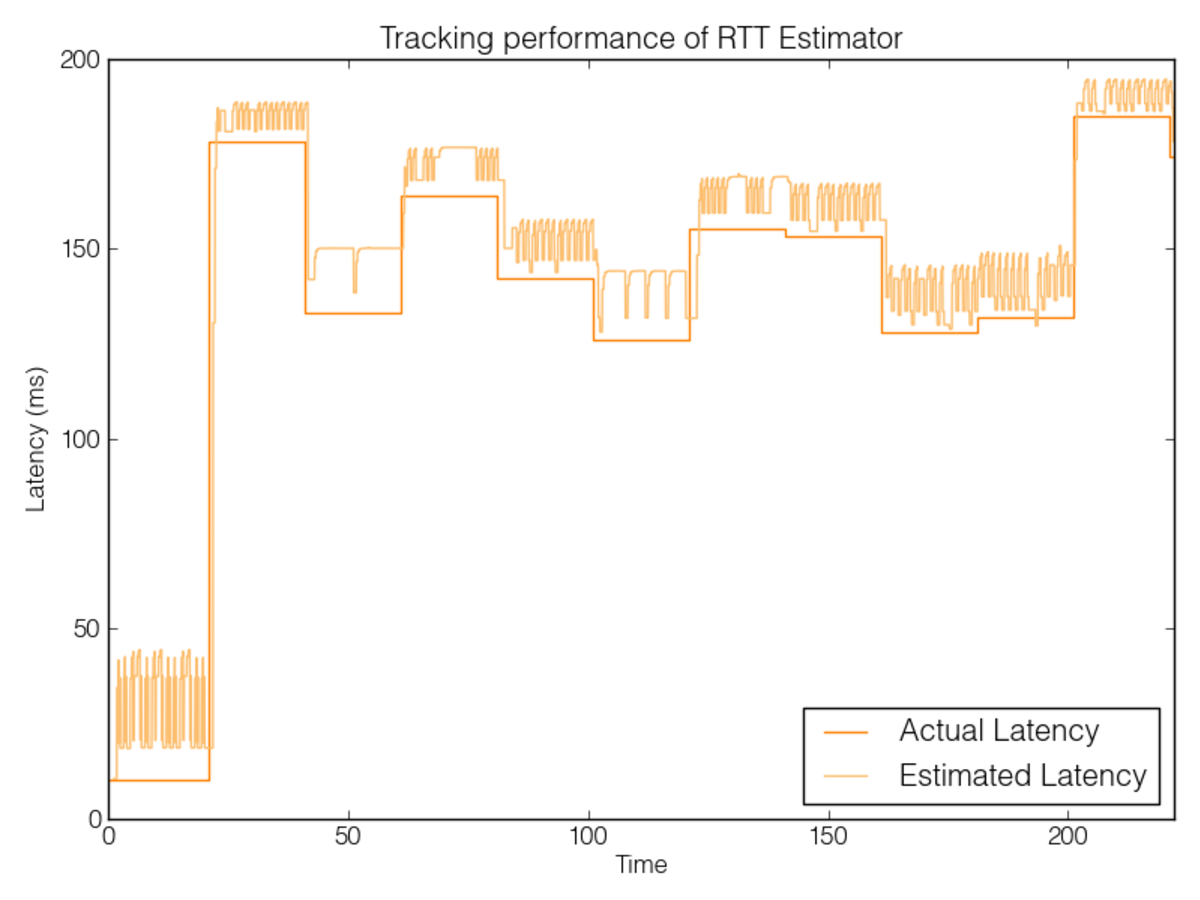
\includegraphics[width=\columnwidth]{track_rtt_final}
\caption{Estimation of latency.}
\label{track_rtt}
\end{center}
\end{figure}

Figure~\ref{track_rtt} shows the difference between the actual latency imposed on our library (simulated using a network wrapper) and the estimate that the system produces.
We use a simple, exponentially-weighted moving average (\ref{ewma}) to track and integrate the round-trip measurements.
\begin{equation}\label{ewma}
Y_n = (\alpha)x_n + (1-\alpha)Y_{n-1}
\end{equation}
Likewise, figure~\ref{track_mtbf} presents real and estimated values for mean-time-between-failure.
Our driver code called shutdown and recover hooks that we placed into the library at random intervals.
To measure MTBF, we store a small sliding window with the times of the last 10 recorded node drop events.
The estimated MTBF is simply the average of these differences.

% Drop tracking
\begin{figure}[htbp]
\begin{center}
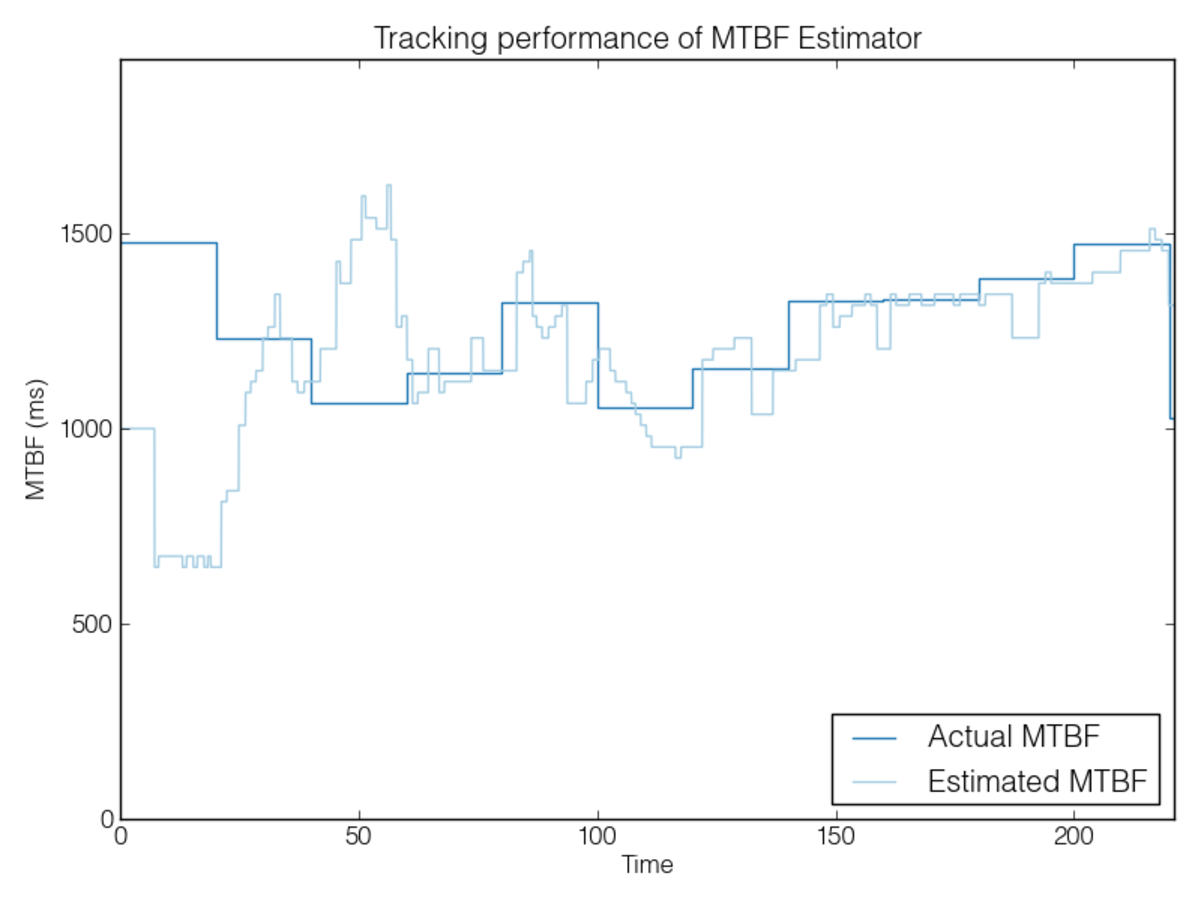
\includegraphics[width=\columnwidth]{track_mtbf_final}
\caption{Estimation of mean time between failure.}
\label{track_mtbf}
\end{center}
\end{figure}

While our latency tracker appears much more precise, this is due to the fact that our experiments were conducted on the same machine (and in point of fact, inside the same process address space).
Our MTBF estimator performs well enough after a burn-in phase---a result of using an un-seeded sliding average.

\subsection{Policy}
Once our data has been gathered, we compute the cost metric presented before from our estimates.
Figure~\ref{track_policy} shows the transitive effects that the errors from our input estimators have on our cost model.
A reasonably stable cost metric is important for maintaining steady-state behavior, and while there are some estimation artifacts (likely due to message pile-up), our estimation is sufficient for our purposes.

% analytical model
\begin{figure}[htbp]
\begin{center}
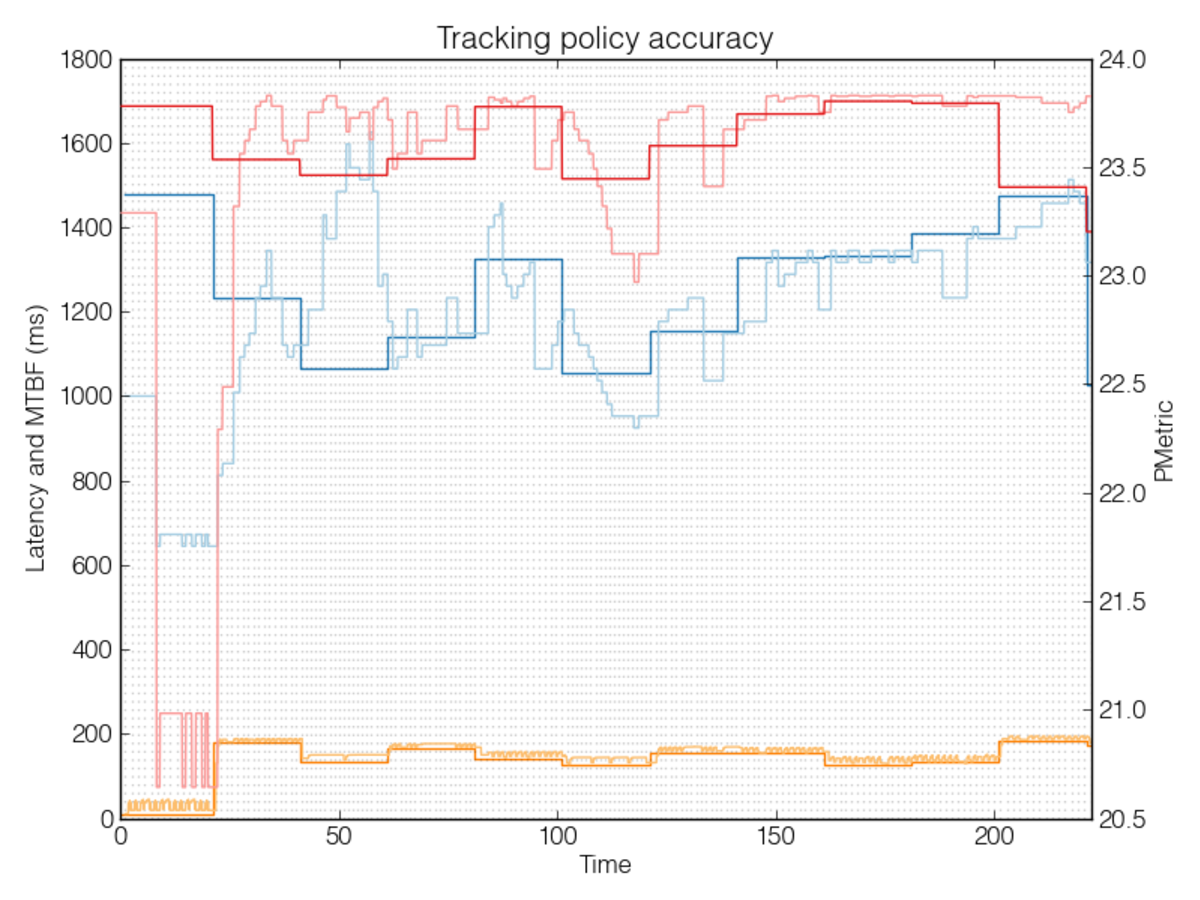
\includegraphics[width=\columnwidth]{track_policy_final}
\caption{Latency tracking is at bottom, in orange, MTBF tracking is in the middle in blue, and the resulting estimate for goodness (PMetric) is shown at top as the light red line. The dark red line represents the same calculation, but computed using exact (oracle) numbers, for reference.}
\label{track_policy}
\end{center}
\end{figure}

The other half of our policy model is a brute-force search algorithm.
In order to identify the best combination of tuning parameters, we exhaustively sweep the parameter space and identify the global maximum (in terms of our estimated PMetric score).
Figure~\ref{search_space} displays a set of parameter curves in this search space.
Here, we are iterating over the node timeout value ($\Tto$) and the heartbeat interval ($\Thb$).
The takeaway here is that while nonlinear, the search space is surprisingly smooth, and (as we describe below), somewhat devoid of saddle points or local maxima.

% parameters
\begin{figure}[htbp]
\begin{center}
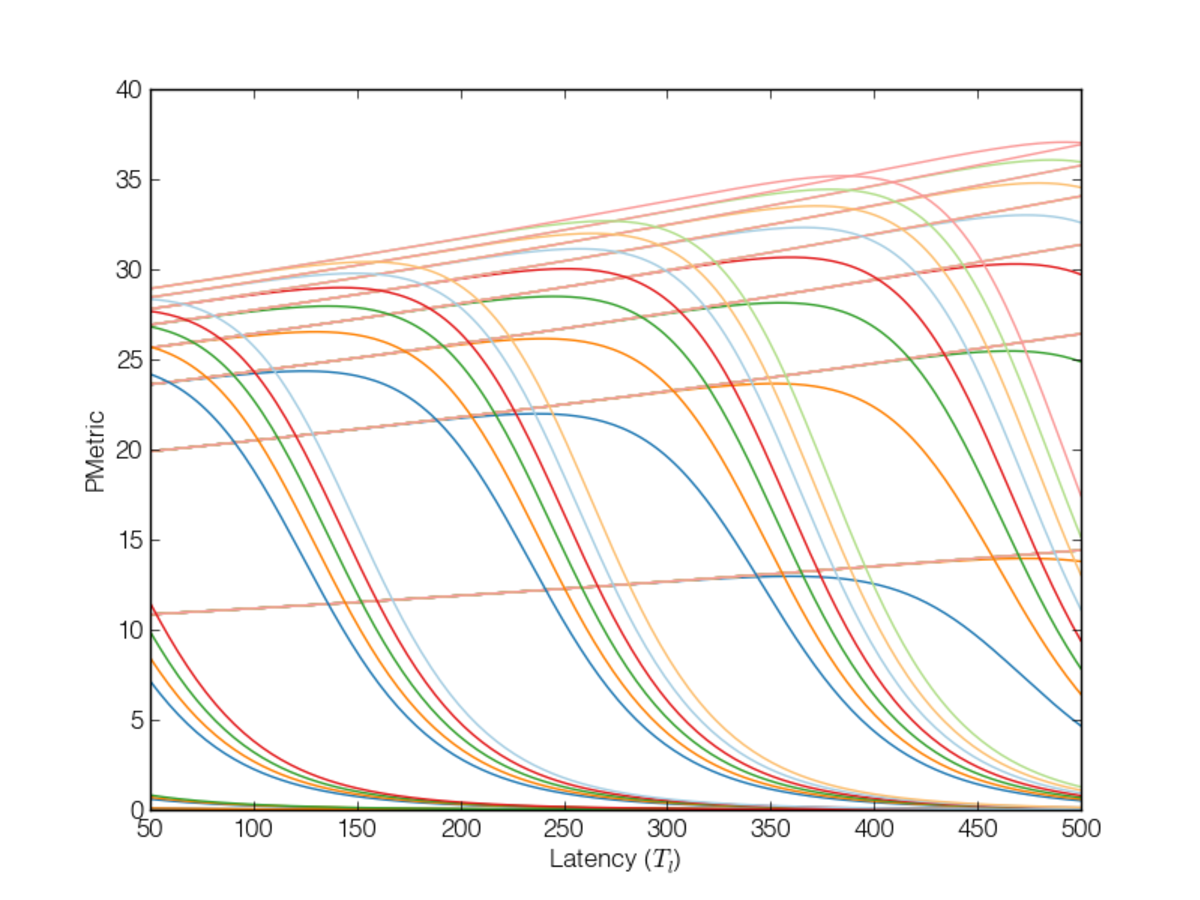
\includegraphics[width=\columnwidth]{search_space_final}
\caption{A 2-dimensional search space.}
\label{search_space}
\end{center}
\end{figure}

\subsection{Tuning}
% monotonic shift
To actually demonstrate the efficacy of our Paxos System in improving its PMetric score, we subjected the Paxos System to a environment with a monotonically increasing latency (Figure~\ref{monotonic_shift}).  As the network becomes worse, the non-adjusting Paxos system should continue to worsen in its PMetric score as well while the autotuning one would be relatively unaffected.  Here, we show that indeed the system which utilizes autotuning does display a higher PMetric for the duration of the experiment, but contrary to our hypothesis, after the initial jump in the PMetric score for the auto tuning system, both PMetric scores track with about the same slope.  This suggests that our chosen PMetric may not be capturing all of the relevant information in the best way to appropriately determine the best parameters for the system.

\begin{figure}[htbp]
\begin{center}
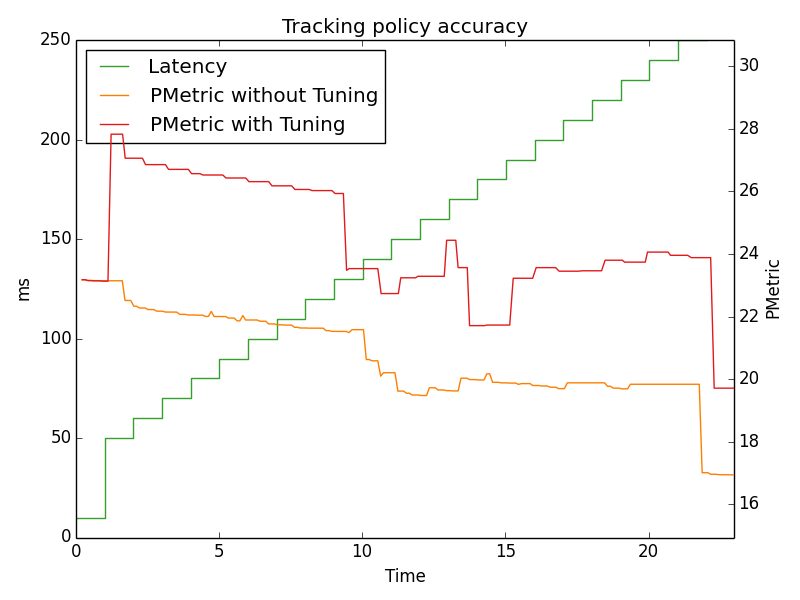
\includegraphics[width=\columnwidth]{monotonic_shift}
\caption{Monotonically Increasing Latency.}
\label{monotonic_shift}
\end{center}
\end{figure}

In order to evaluate how well our system adjusts to latency to improve its performance, we measured the system's goodput by determining the time it takes for our system to serve a fixed number of client requests where each request requires a full instance of Paxos.  Figure~\ref{goodput} shows how well a system using autotuning compares to one that does not in terms of its goodput with monotonically increasing network latency.  For the most part, both systems track very well in terms of how their goodputs change with changing latency implying further that our PMetric does not catch the interesting network metrics in the most significant way to make the best parameter decisions; however, there is a point in time when the latency gets relatively large where the system using autotuning \emph{does} perform better than the one which does not.  This suggests that what our PMetric measures most is elements of the system that make the most difference in extreme environments.  

\begin{figure}[htbp]
\begin{center}
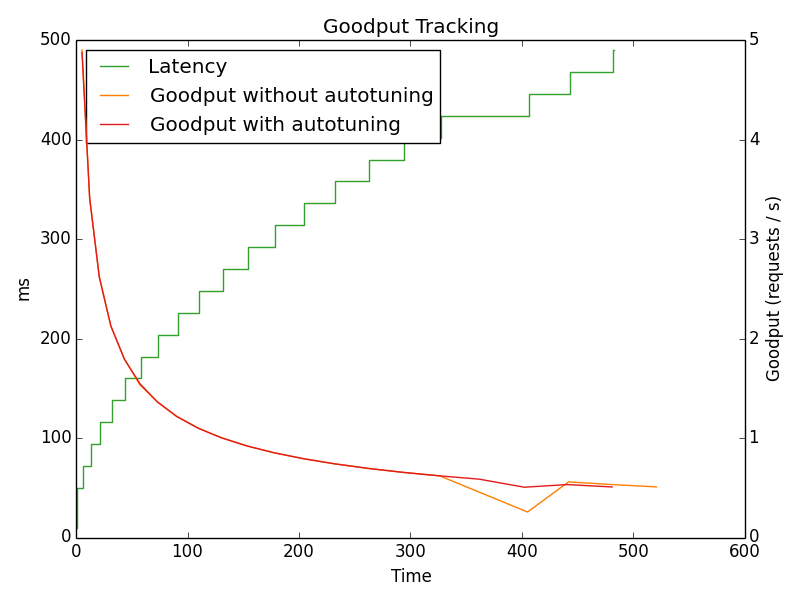
\includegraphics[width=\columnwidth]{goodput}
\caption{Measuring Goodput with a Changing Latency.}
\label{goodput}
\end{center}
\end{figure}